% !TEX root = ../../prj4projektdokumentation.tex

\section{Kontrolmodul}

Kontrolmodulet består primært af to processer; En kommunikationsdel der kan håndtere at modtage data gennem en TCP forbindelse og konvertere disse data til noget der kan bruges i resten af programmet, herunder også HMI delen. En styringsdel der kan bruge disse data i styringen af trinskifteren.

\subsection{TCP kommunikation}
Kontorlmodulet er lavet som en client i forhold til kommunikationsmodulet, der er server. Den sender altså en forespørgelse på at modtage data til kommunikationsmodulet, hvorefter den modtager ny data fra den forespurgte enhed. Mere om selve protokollen kan findes i afsnit \ref{TCPprotokol} TCP protokol. Det er kontrolmodulet der oprette TCP forbindelse og står for at nedlægge den igen. \\
TCP komunikationen er opdelt i 4 FC'er; OpretForbindelse, SendData, ModtagData og AfslutForbindelse. Simatic TIA portal har nogle indbyggede blokke, man bruger når til Ethernetkommunikation. \\
OpretForbindelse består af funktionsblokken TCON, som er vist på figur \ref{fig:TCON}. Når REQ får et 1, vil den forsøge at forbindelse til en bestemt IP adresse og opretholde den, også selvom REQ bliver sat 0. Forbindelse bliver vedligeholdt automatisk asynkront, så programmet kan udføre andet samtidigt. \\
ID er identifikationen på forbindelsen internt i PLC'en, som de resterende blokke bruger til at identificere hvilken forbindelse er tilknyttet, hvis der skulle være flere. Her ID sat til 1, da der kun er en forbindelse til kommunikationsmodulet.
CONNECT parameteren er en pointer til data området der indeholder forbindelsesinformation. Blokken muliggør at få informationer om forbindelsen tilstand gennem DONE, BUSY, ERROR og STATUS. I dette projekt er der dog ikke udviklet nogen form for fejlhåndtering og disse er ikke brugt. Der henvises til !!!!SYSTEM MANUAL REFERNCE!!!! for mere dybdegående forklaring af disse.

\begin{figure}[H] % (alternativt [H])
	\centering
	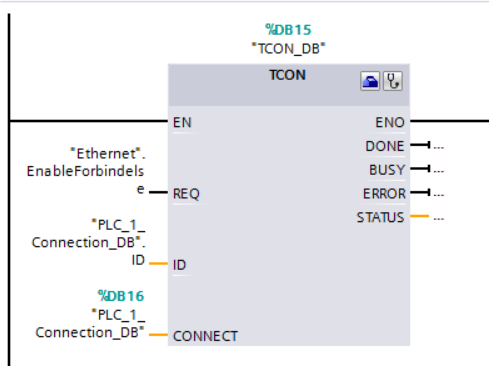
\includegraphics[width=0.5\textwidth]{Figure/TCON}
	\caption{TCON brugt i funktionen OpretForbindelse}
	\label{fig:TCON}
\end{figure}


\begin{figure}[H] % (alternativt [H])
	\centering
	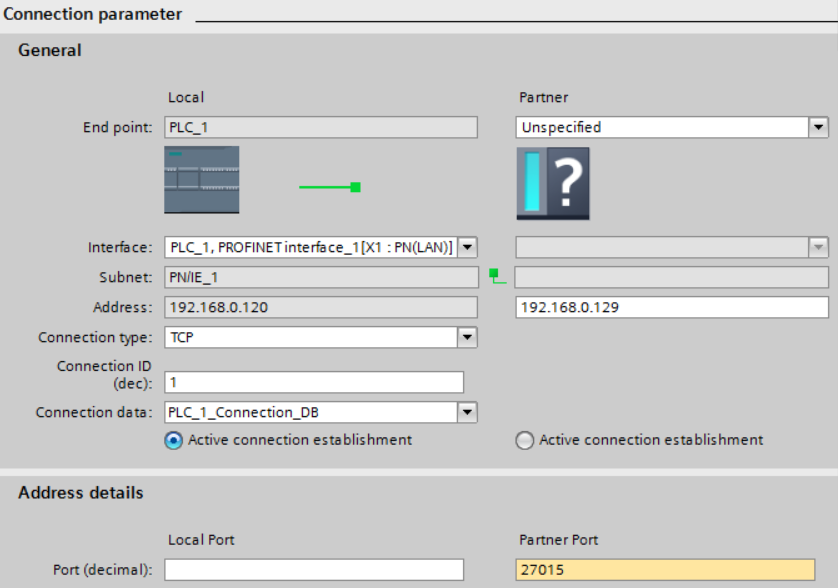
\includegraphics[width=0.5\textwidth]{Figure/KonfigurationAfTCPforbindelse}
	\caption{Konfiguration af TCP forbindelse}
	\label{fig:Konfiguration}
\end{figure}

\begin{figure}[H] % (alternativt [H])
	\centering
	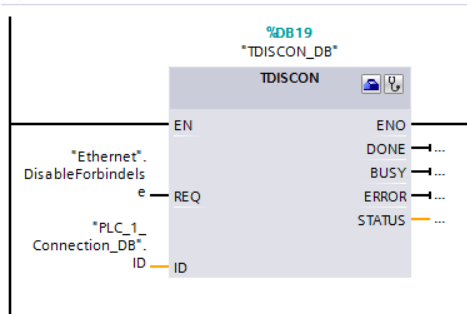
\includegraphics[width=0.5\textwidth]{Figure/TDISCON}
	\caption{TDISCON brugt i funktionen AfslutForbindelse}
	\label{fig:TDISCON}
\end{figure}

\begin{figure}[H] % (alternativt [H])
	\centering
	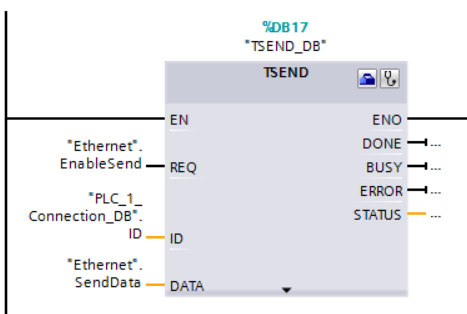
\includegraphics[width=0.5\textwidth]{Figure/TSEND}
	\caption{TSEND brugt i funktionen SendData}
	\label{fig:TSEND}
\end{figure}

\begin{figure}[H] % (alternativt [H])
	\centering
	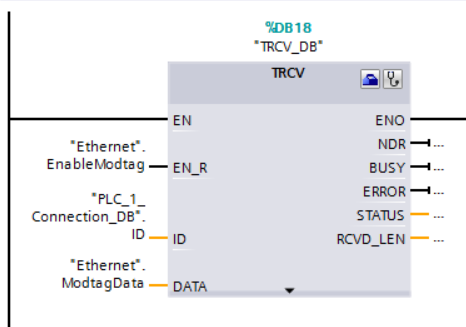
\includegraphics[width=0.5\textwidth]{Figure/TRCV}
	\caption{TRCV brugt i funktionen ModtagData}
	\label{fig:TRCV}
\end{figure}


\subsection{Styring af trinskifter}